\documentclass[12pt]{article}
 
\usepackage[margin=1in]{geometry} 
\usepackage{amsmath,amsthm,amssymb, graphicx, multicol, array}
\usepackage{parskip}
\usepackage{booktabs}


 \usepackage{amsmath}
\usepackage{amsfonts}
\usepackage{amssymb}
\usepackage[version=4]{mhchem}
\usepackage{stmaryrd}
\usepackage[margin=1in]{geometry} 
\usepackage{amsmath,amsthm,amssymb, graphicx, multicol, array}
\usepackage{parskip}
\usepackage{booktabs}

 
\newcommand{\N}{\mathbb{N}}
\newcommand{\Z}{\mathbb{Z}}
 

\begin{document}
 
\title{Problem Set 3}
\author{Nicolas Moreno, Kushal Patel, Olivia Wilkinson \\
ECON: 880}
\maketitle

\section{Exercise 1}
Solve the dynamic programming problem of retirees and workers. Plot the value function over a for a retired agent at the model-age 50. Is it increasing and concave? Plot the savings function for a worker at the
model-age 20, $a'_{20}(z, a)$. Is saving increasing in a? Is it increasing in z?

\begin{figure}[h!]
    \centering
    \caption{Age Efficiency Profile}
    \vspace{1cm}
    \includegraphics[width=0.75\linewidth]{PS5_graphs/q1_η.png}
    
    \label{fig:ageefficiency}
\end{figure}

Figure \ref{fig:ageefficiency} shows the age efficiency profile, $\eta$. Figure \ref{fig:val50} shows the value function is increasing and concave for the retired agent. 
\newpage

\begin{figure}[h!]
    \centering
    \caption{Model-ages 50 and 20 Value Functions}
    \vspace{1cm}
    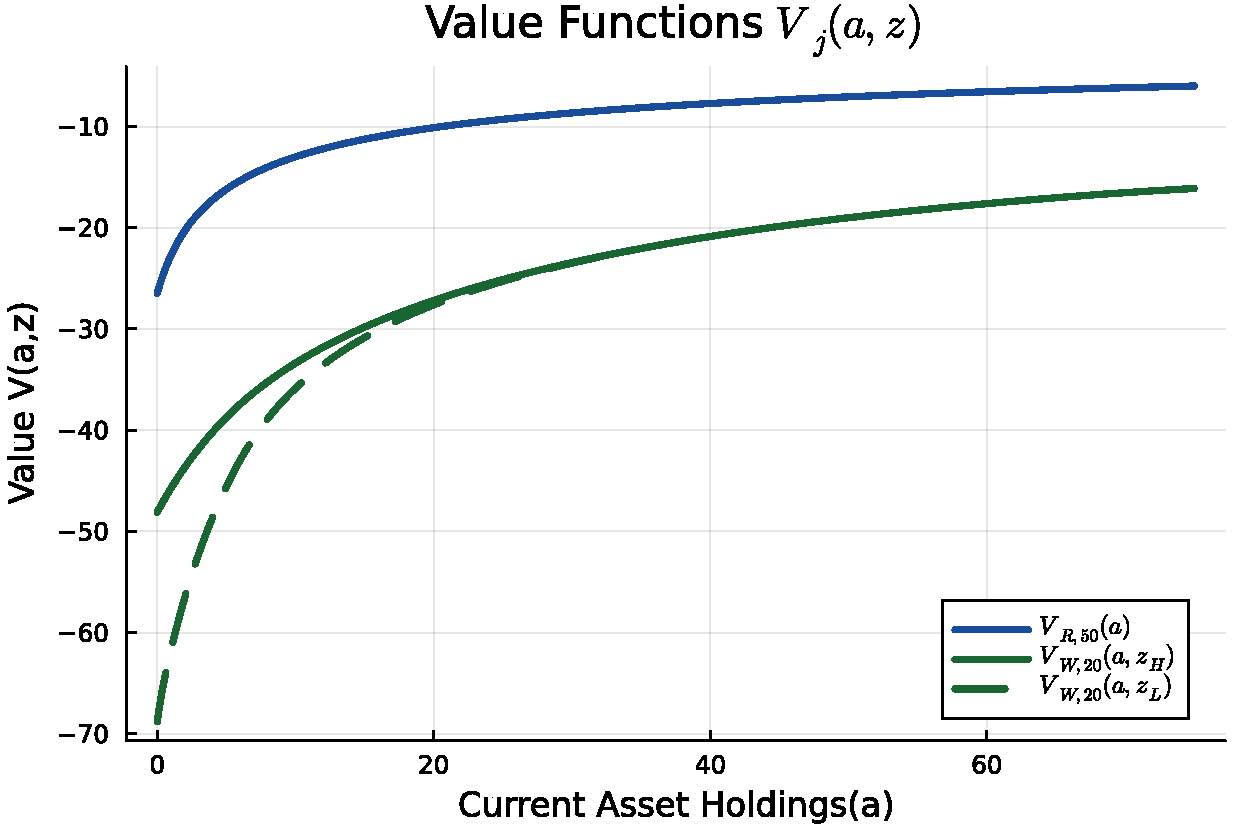
\includegraphics[scale=0.5]{PS5_graphs/Value_Functions.pdf}
    
    \label{fig:val50}
\end{figure}

Figure \ref{fig:pol20} shows the policy function for a worker at model age 20. Asset choice is increasing in assets. Figure \ref{fig:pol_change20} shows the savings function. Up until a certain level of assets, savings is higher for high productivity workers. Savings is decreasing in assets for high productivity workers until assets are approximately 45 then increasing. Savings are continuously increasing for low productivity workers. The drop-off in the graph towards the end of the asset grid is due to the asset grid bounds. 
\\

\begin{figure}[h!]
    \centering
    \caption{Savings choice model age 20}
    \vspace{1cm}
    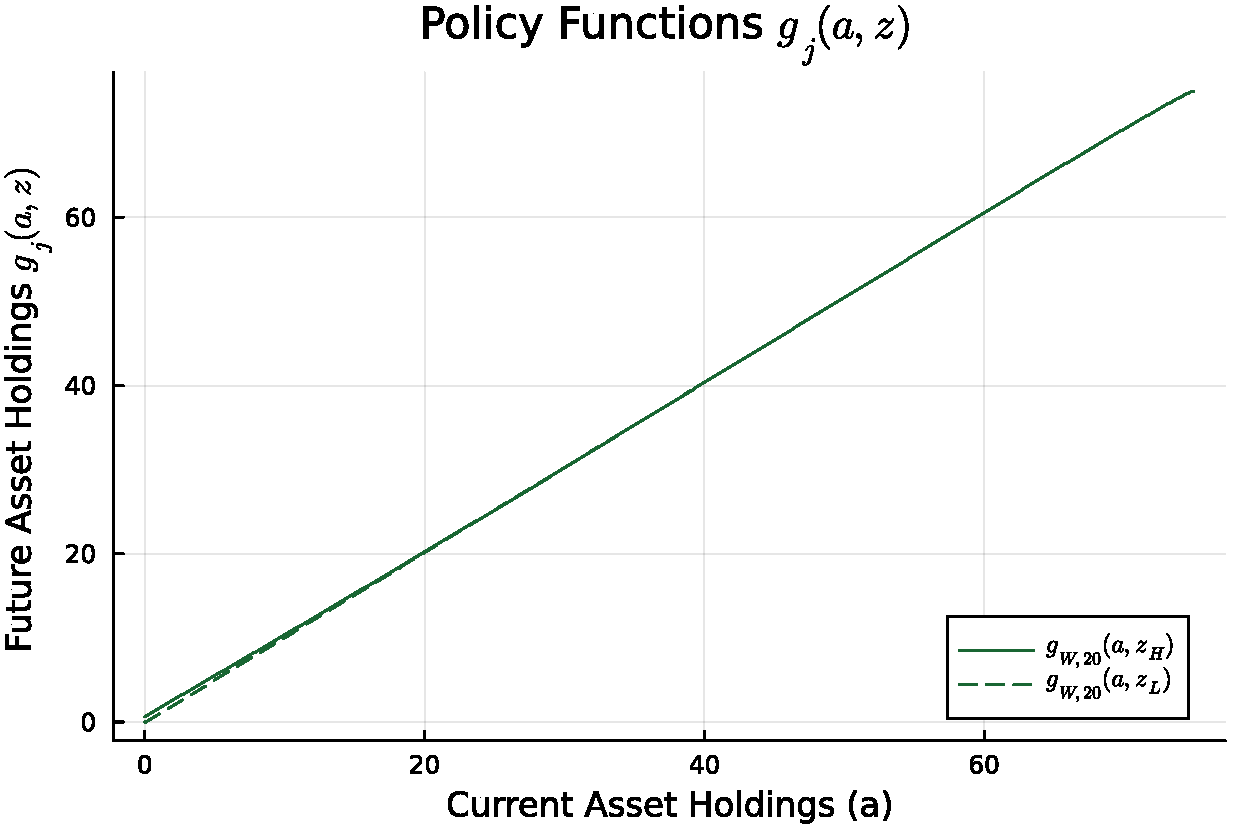
\includegraphics[scale=0.5]{Computational/ECON 880 Q1/PS5_graphs/Policy_Functions_Workers.pdf}
    
    \label{fig:pol20}
\end{figure}

\begin{figure}[h!]
    \centering
    \caption{Change in savings model age 20}
    \vspace{1cm}
    \includegraphics[width=0.75\linewidth]{PS5_graphs/q1_polfunc_δ_20.png}
    
    \label{fig:pol_change20}
\end{figure}

\newpage
\section{Counterfactuals}

Table \ref{tab:policyres} shows the results of the policy counterfactual experiments. The first column shows the benchmark economy first with social security and then without. The second column shows the economy with no productivity risk in the same order. Finally the third column shows the economy with exogenous labor choice? 

\begin{table}[h!]
    \centering
    \begin{tabular}{|c|c|c|c|c|c|c|}
    \hline
         & \multicolumn{2}{c|}{Benchmark} & \multicolumn{2}{c|}{No Risk} & \multicolumn{2}{c|}{Exogenous Labor} \\
         \hline 
         & with ss & no ss & with ss & no ss & with ss & no ss \\
         \hline
         capital $K$ & 3.39 & 4.77 & 0.97 & 1.29 & 7.25 & 10.49 \\
         labor $L$ & 0.34 & 0.37 & 0.16 & 0.18 & 0.75 & 0.75 \\
         wage $w$  & 1.46 & 1.61 & 1.22 & 1.31 & 1.49 & 1.65 \\
         interest $r$ & 0.02 & 0.01 & 0.05 & 0.04 & 0.02 & 0.01\\
         pension benefit $b$ & 0.26 & 0.00 & 0.09 & 0.00 & 0.49 & 0.00 \\
         total welfare $W$ & -35.8 & -37.2 & -46.5 & -45.9 & -23.6 & -25.8\\
         cv(wealth) & 0.60 & 0.70 & 0.98 & 0.88 & 0.59 & 0.71 \\
         \hline 
    \end{tabular}
    \caption{Policy experiment results }
    \label{tab:policyres}
\end{table}

\begin{enumerate}
    \item First, solve for the benchmark model with social security. Is this economy dynamically efficient (compare the interest rate with the implicit return from social security, which is equal to the population growth rate)? Now eliminate social security by setting $\theta = 0$. Observe how aggregate capital accumulation and labor supply change as a result of the tax reform. Provide intuition in terms of insurance and output efficiency. How does aggregate welfare change? Who benefits and who loses due to this reform? How does the reform affect cross-sectional wealth inequality? You can use table 1 to support your answers.

    Yes the economy is dynamically efficient since the interest rate (2\%) is greater than the population growth rate (1.1\%). When social security is eliminated, aggregate labor and capital (savings) grow since workers need to save more for retirement without the pension benefit. The extra savings cause the interest rate to decline to about 1\%. Aggregate welfare declines from -35.8 to -37.2 and increases wealth inequality. 

    
    \item In the second experiment, there is no idiosyncratic risk. Assume that at each age j, $z_L$ = $z_H$ = 0.5. First, compute the aggregate variables for the case with social security. How does the aggregate capital stock change relative to the benchmark model? Provide intuition in terms of capital as a buffer stock. Then, eliminate social security. How does the aggregate welfare change? What can you conclude about social security as an insurance device against idiosyncratic risk? Comment on the extent, to which these welfare comparisons across steady states are meaningful or misleading.

    Capital stock declines from 3.39 to 0.97 since workers are all low productivity and no longer have to save for negative productivity shocks. As a result of the decline in savings, the interest rate rises to 5\%. However, aggregate labor supply, wage, and the pension benefit are smaller in the no-risk economy compared to the benchmark and total welfare is lower. When social security is eliminated, aggregate welfare increases in the no risk economy. The capital stock increases, aggregate labor increases slightly, wages rise, the interest rate declines, and wealth inequality reduces. This suggests that social security is not beneficial in economies with no idiosyncratic risk. A main benefit of the pension is having a steady source of income when old regardless of productivity's when young, so in the economy with idiosyncratic risk, social security helped to reduce wealth inequality by reducing savings of the high productivity workers. In the economy with no idiosyncratic risk, we no longer have this additional benefit. Also, since social security is financed through a distortionary labor tax, it reduces labor supply and therefore production, which is already in shorter supply in the low-productivity-no-risk economy. Still, we must be careful comparing welfare across steady states because we do not have information about the transition path taken to reach the new steady state. When social security is first eliminated, workers near retirement and the retired group do not have enough time to accumulate savings for consumption smoothing and will be worse off without the social security. 
   
    \item Consider the case, when labor supply is exogenous ($\gamma = 1$). Compare the distortionary effect of social security on the aggregate labor supply. How does the support for social security change with exogenous labor supply?

    With exogenous labor supply, there is no disutility of labor and asset choice does not effect labor supply. As a result, aggregate labor is unchanged when social security is eliminated in this version of the economy. Total welfare is higher and wealth inequality is lower with social security so it is beneficial in this case. 

    
\end{enumerate}

\end{document}